\documentclass[11pt]{amsart}
\usepackage[margin=1in]{geometry} 
%\geometry{landscape}                % Activate for for rotated page geometry
\usepackage[parfill]{parskip}    % Activate to begin paragraphs with an empty line rather than an indent
\usepackage{graphicx}
\usepackage{rsfso}% so \mathcal uses acute rsfs
\usepackage{mathrsfs}% so \mathscr uses natural rsfs

\title{An acute script font based on RSFS}
\author{Michael Sharpe}
\email{msharpe at ucsd dot edu}
%\date{}                                           % Activate to display a given date or no date

\begin{document}
\maketitle
The {\tt rsfs} fonts are, in their natural states, very oblique, appearing to be slanted to the right at close to 45$^\circ$. In my opinion, this makes them less suited for use as a replacement for \verb|\mathcal|. (The \verb|\mathrsfs| package defines \verb|\mathscr| to use {\tt rsfs} for output.)

The purpose of this package is to make a collection of virtual fonts from the {\tt rsfs} PostScript fonts that remove much of the slant. The {\tt o} in {\tt rsfso} stands for {\tt oblique}, though {\tt acute} would be a better description.  The end result is quite similar in appearance, modulo a few flourishes, to the commercial script font in the Adobe Mathematical Pi collection. Here is a sample (as a png snapshot) of the latter, produced via \verb|\usepackage[mathcal]{mathpi}|.

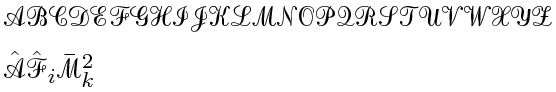
\includegraphics{mh2scr0}

The second line above shows that work will need to be performed to get spacing, accents and subscript positions in better shape than when invoked by the now obsolete {\tt mathpi} package. The same fragment using {\tt rsfso} renders as

$\mathcal{ABCDEFGHIJKLMNOPQRSTUVWXYZ}$

$\mathcal{\hat{A}}\mathcal{\hat{F}}_i\mathcal{\bar{M}}^2_k$

and with {\tt mathrsfs} you get

$\mathscr{ABCDEFGHIJKLMNOPQRSTUVWXYZ}$

$\mathscr{\hat{A}}\mathscr{\hat{F}}_i\mathscr{\bar{M}}^2_k$

The {\tt rsfso} package has two options: {\tt scr} causes a redefinition of \verb|\mathscr| rather than \verb|\mathcal|, and {\tt [scaled=1.1]} expands the size by a factor of 1.1, allowing you to match the size of the \verb|\mathcal| (or \verb|\mathscr|) output to your math font.

The virtual font production and their metric adjustments were carried out using the author's freely available OS X program {\tt TeXFontUtility} which serves, among other functions, as a visual front-end to some {\tt fontinst} manipulations.

\end{document}  
